% =====================================================================
% Dataset sample grid. Source: annotated frames from LuggageDataset v6i,
% as presented in our EUSIPCO submission; reproduced here WITHOUT the
% augmentation pipeline used there.
% =====================================================================
\begin{figure}[t]
\centering
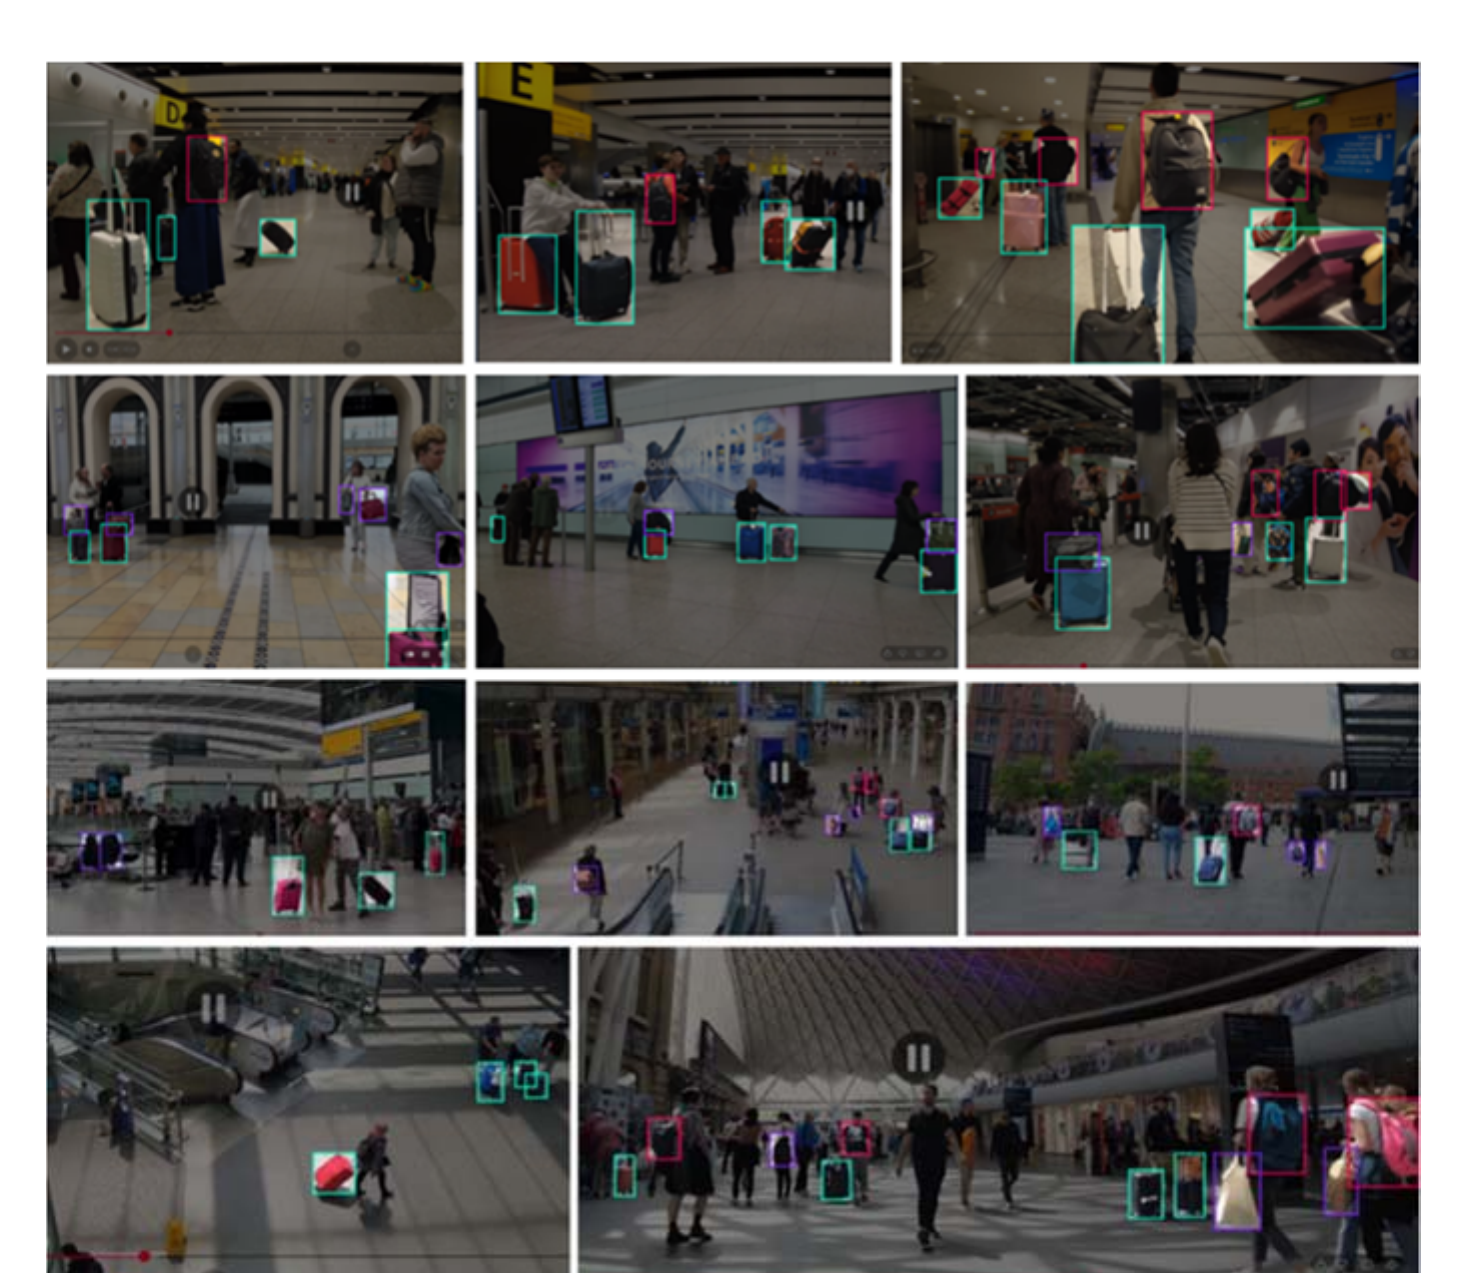
\includegraphics[width=\linewidth]{fig_samples.png}
\caption{Representative annotated frames from LuggageDataset~v6i. The images are
drawn from fixed or quasi-static surveillance cameras in transport hubs and
indoor public space, and illustrate the conditions the benchmark is built to
capture: elevated, oblique viewpoints in which luggage occupies a small fraction
of the frame; dense pedestrian traffic with frequent partial occlusion of the
bag by its own owner; wide variation in illumination, from daylit concourses to
artificially lit interiors and screen-lit walls; and all three classes
co-occurring at very different apparent scales within a single frame. The
annotations shown are the released ground truth. Note that these are the raw
frames: unlike our earlier presentation of this corpus, no augmentation is
applied anywhere in this paper, so every number reported in
Section~\ref{sec:results} is obtained on unmodified imagery.}
\label{fig:samples}
\end{figure}
